In this section, I will provide logical explaination and statistical results,
illustrated as figures or tables, to address research questions mentioned in
\autoref{sec:research_questions}.

\subsection{RQ1: What types of stolen information are traded?}
As shown in \autoref{fig:type_allocation}, I captured in total 10 product types
based on my own standard. Among all categories, \emph{Personal Data} is the
most active field, contributing \(68,69\%\) of all traded items. \emph{Online Account}
represents the second larges portion \(17,73\%\). The rest of product types ranges
from \(0,36\%\) to \(3,64\%\). Detailed description of each product type is in
\autoref{tab:category_description}.

\begin{table}
    \centering
    \begin{tabular}{|c|c|}
        \hline
        Product type & Description\\
        Personal Data & Full name, date of birth, social security number, home
        address, zip code, driver license, employer info, etc.\\
        Online Account & online account of services such as Netflix, Amazon,
        Venmo, Booking.com, etc.\\
        Bank Account & Username/password of online bank accounts, and credential
        information linked to bank accounts.\\
        Credit Card & card holder name, \acrshort{cvv}, full name, address,
        bank name, card type.\\
        Passport & Real photos and scan of passports.\\
        Email & Emails leaked through data breaches.\\
        Lookup Service & \acrshort{ssn}/\acrshort{dob}/\acrshort{mmn}/\acrshort{dl}
        /\acrshort{cs} lookup service.\\
        Bank Identity Number & \acrshort{bin} is the first 6 digits of the credit card (with
        the help of this information you will understand what credit cards you need to
        work with 3-D Secure VBV) 3-D Secure VBV is a protocol that is used as an
        additional layer of security for online credit and debit cards, two-factor
        user authentication.\\
        Remote Desktop Protocol & The protocol provides user graphical interface to connect
        to other computers over the network connection \cite{web:rdp_wiki}.\\
        Other & Tutorials, digital document templates, document forms, domains, etc.\\
        \hline
    \end{tabular}
    \caption{Description of product types.}\label{tab:category_description}
\end{table}

\subsection{RQ2: What are the prices for different product types?}

\begin{figure}
    \centering
    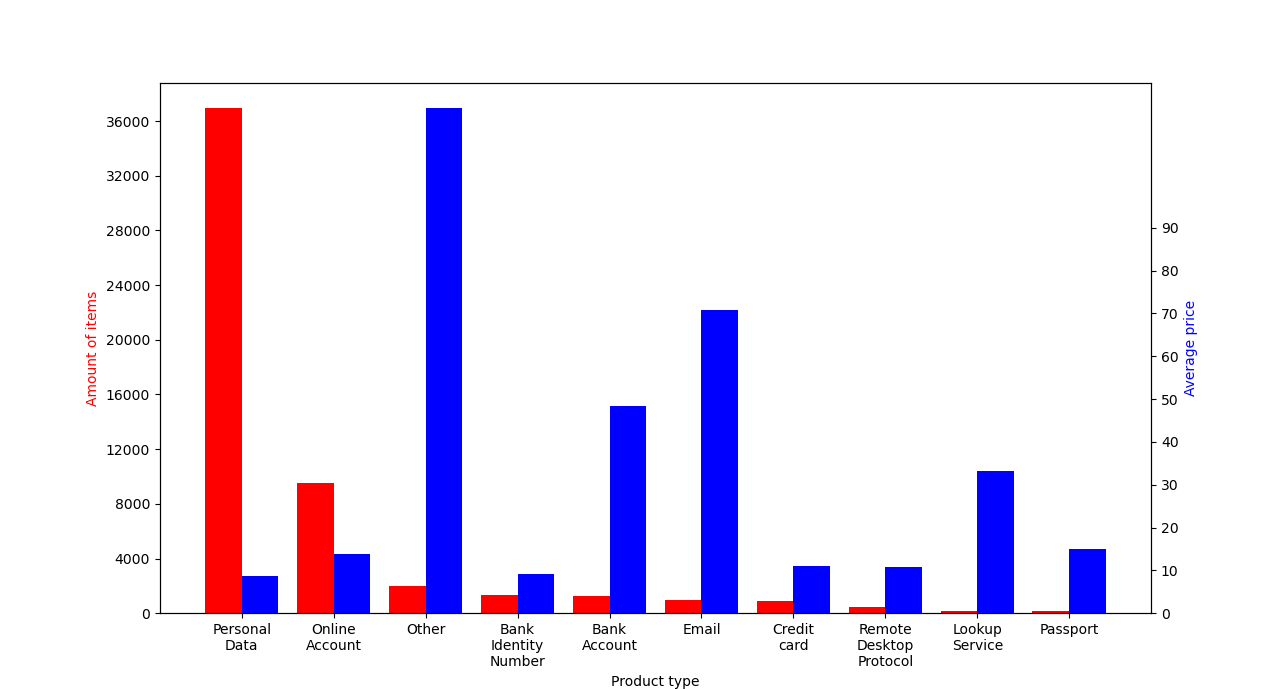
\includegraphics[height=\textheight,width=\textwidth,keepaspectratio]
    {plots/cate_prods_avg_price.png}
    \caption{Number of products and average price over product types.}
    \label{fig:cate_avg_prod}
\end{figure}

\subsection{RQ3: Where the stolen information is from?}

\subsection{RQ4: What we can learn about the sellers?}